\begin{mdframed}[style=warning]
	\begin{ejercicio}
		\textbf{Conceptos: }
		\begin{enumerate}[a)]
			\item Compare la ley de Ampère con la ley de Biot$-$Savart. ¿Cuál es generalmente la más útil para calcular $\vec{B}$ en un conductor que trasnporta corriente?
			\item ¿Es válida la Ley de Ampère para todas las trayectorias cerradas que rodean un conductor?
		\end{enumerate}
	\end{ejercicio}
\end{mdframed}











\begin{mdframed}[style=warning]
	\begin{ejercicio}
		Encuentre la fuerza sobre cada una de las espiras mostradas en la figura. Tanto el cable infinito, como las espiras tienen una corriente $I$.
		\begin{figure}[H]
			\centering
			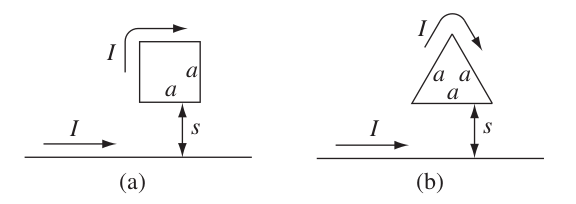
\includegraphics[scale=0.5]{./img/p1.png}
			\caption{Espiras.}
			\label{espiras}	
		\end{figure}
	\end{ejercicio}
\end{mdframed}


















\begin{mdframed}[style=warning]
	\begin{ejercicio}
		Suponga que se tienen dos líneas de carga $\lambda$, separadas una distancia $d$, moviendose a una velocidad $v$. Qué tan grande debería ser $v$ para que la fuerza magnética de atracción se equipare a la fuerza eléctrica de repulsión? Encuentre el valor numérico. Es un resultado razonable?
		\begin{figure}[H]
			\centering
			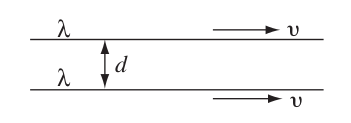
\includegraphics[scale=0.5]{./img/p2.png}
			\caption{Líneas de Carga.}
			\label{DF}	
		\end{figure}
	\end{ejercicio}
\end{mdframed}
























\begin{mdframed}[style=warning]
	\begin{ejercicio}
		Dos bobinas circulares son coplanares (sobre el plano $xy$) y transportan la misma magnitud de corriente $i$ en la misma dirección. Sus ejes están alineados con el eje $z$. La bobina grande (radio $R$ y $N$ vueltas) está fijada en un soporte y no se mueve, mientras la bobina pequeña de radio $r \ll R$ (solo $1$ vuelta) está fija en el eje $z$, pero tiene libertad de movimiento en el plano $xy$. El material del alambre del que está fabricado la bobina pequeña tiene un módulo de elasticidad $Y$ y tiene sección transversal $A$. Determine (despreciando la fuerza de gravedad), en términos de $\mu _o$, $i$, $R$, $r$, $N$, $Y$ y $A$:
		\begin{enumerate}[a)]
			\item Una expresión para el vector de campo magnético causado por una bobina grande en la bobina pequeña. Asuma $(R-r) \sim R$.
			\item Una expresión para la magnitud de la fuerza neta que siente la bobina pequeña. En el resultado final, no simplifique la condición $r \ll R$; simplemente deje indicado el resultado en términos de ambas variables.
			\item Si la bobina pequeña no debe sufrir una deformación unitaria mayor a $E$, escriba una expresión para determinar la sección transversal mínima del alambre.
		\end{enumerate}
		\begin{figure}[H]
			\centering
			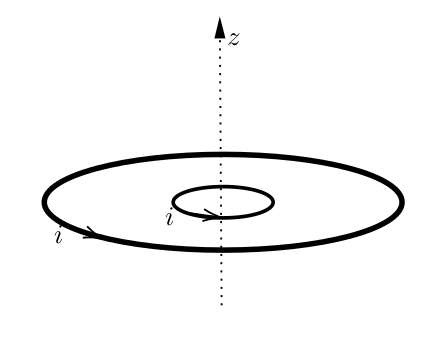
\includegraphics[scale=0.5]{./img/p4.png}
			\caption{Espiras concentricas.}
			\label{DF}	
		\end{figure}
	\end{ejercicio}
\end{mdframed}


















\begin{mdframed}[style=warning]
	\begin{ejercicio}
		Una corriente estacionaria $I$ fluye por un cilindro de radio $a$. Encuentre el campo magnetico dentro y fuera del cilindro si: la corriente es distribuída uniformemente por la superficie exterior del cable y si la corriente está distribuída de una forma que $J$ sea proporcional a $s$ (distancia desde el eje).
		\begin{figure}[H]
			\centering
			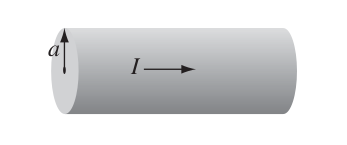
\includegraphics[scale=0.5]{./img/p5.png}
			\caption{Cable cilíndrico.}
			\label{DF}	
		\end{figure}
	\end{ejercicio}
\end{mdframed}




























\begin{mdframed}[style=warning]
	\begin{ejercicio}
		Una losa gruesa extendida como se muestra en la figura (infinita en las direcciones $x$ e $y$). Esta losa carga una densidad de corriente volumétrica uniforme $\vb{J} = J\vx$. Encuentre el campo magnético en función de $z$, dentro y fuera de la losa.
		\begin{figure}[H]
			\centering
			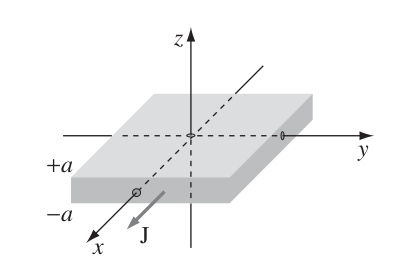
\includegraphics[scale=0.5]{./img/p3.png}
			\caption{Losa con densidad de corriente $\vb{J}$.}
			\label{DF}	
		\end{figure}
	\end{ejercicio}
\end{mdframed}




















%%%%%


















































%%%